\documentclass[letterpaper,11pt,twoside]{article}
\usepackage[margin=0.88in]{geometry}
\usepackage{xcolor}

%%%%%%%%%%%%%%%%%%%%%%%%%%%%%%%%%%%%%%%%%%%%%%%%%%%%%%%%%%%%%%%%%%%%%%%%%%%%%%%


\def\mypdfauthor{Dimitris Diochnos}
\def\mypdfsubject{Undergraduate Course}
\def\mypdftitle{CS 3823 - Theory of Computation, 2025F: HW1}
\def\myheadertitle{CS 3823 - Theory of Computation: Homework Assignment 1}
\def\mytitle{CS 3823 - Theory of Computation: Homework Assignment 1}
\def\thecurrentsemester{Fall 2025}
\def\myduedate{\textbf{Due:} Friday, September 12, 2025}


%%%%%%%%%%%%%%%%%%%%%%%%%%%%%%%%%%%%%%%%%%%%%%%%%%%%%%%%%%%%%%%%%%%%%%%%%%%%%%%


\usepackage{xspace}
\usepackage{enumitem}
%\usepackage[numbers,square,sectionbib,sort&compress]{natbib}
\usepackage[numbers,square,sort&compress]{natbib}
\usepackage[euler-digits, T1]{eulervm}
\usepackage{upgreek}
\usepackage[dvipsnames]{xcolor}
\usepackage[
   colorlinks%
   ,plainpages=false%This forces a unique identification of pages.
   ,hypertexnames=true%This is necessary to have exact link on Index page.
   ,naturalnames
   ,hyperindex
   ,citecolor=OliveGreen
   ,urlcolor=RoyalBlue
   ,pdfauthor={\mypdfauthor}
   ,pdftitle={\mypdftitle}
   ,pdfsubject={\mypdfsubject}
   %,pdfkeywords={...}
]{hyperref}
%\usepackage{lettrine}
%\input{definitions}
\usepackage{psfrag}
\usepackage{graphicx}
\usepackage{multirow}
\usepackage{multicol}
%\usepackage{vwcol}
\usepackage{enumitem}

%%%%%%%%%%%%%%%%%%%%%%%%%%%%%%%%%%%%%%%%%%%%%%%%%%%%%%%%%%%%%%%%%%%

\usepackage{bm}
\usepackage{pstricks}
\psset{unit=0.45cm}
\psset{linewidth=0.05}%
\psset{fillstyle=solid}%

\newcommand{\sample}{\ensuremath{S}\xspace}
\newcommand{\XX}{\ensuremath{\mathcal{X}}\xspace} % X

%%%%%%%%%%%%%%%%%%%%%%%%%%%%%%%%%%%%%%%%%%%%%%%%%%%%%%%%%%%%%%%%%%%

\usepackage{fancyhdr}
\pagestyle{fancy}
\usepackage{lastpage}

\setlength{\headheight}{14pt}

\fancypagestyle{firststyle}
{
   \fancyhf{}
   \fancyfoot[L]{\today}
   %\fancyfoot[C]{\thepage/\pageref*{LastPage}}
   \fancyfoot[R]{\thepage/\pageref*{LastPage}}
}


\newcommand{\stylishPagesColor}{Gray}
\newcommand{\stylishHref}[2]%
{\hypersetup{urlcolor=\stylishPagesColor}%
\href{#1}{#2}%
\hypersetup{urlcolor=RoyalBlue}}


\fancyhead{} % clear all header fields
\fancyhead[CO,CE]{\textsc{\myheadertitle}}
\fancyfoot{} % clear all footer fields
\fancyfoot[LO,RE]{\today}
\fancyfoot[RO,LE]{\thepage/\pageref*{LastPage}}
\renewcommand{\headrulewidth}{0.0pt}
\renewcommand{\footrulewidth}{0.0pt}

% So that absolute values and norms are neat.
\usepackage{amsmath}
\providecommand{\abs}[1]{\lvert#1\rvert}
\providecommand{\norm}[1]{\lVert#1\rVert}

\newcommand{\OO}[1]{\ensuremath{\mathcal O\left(#1\right)}\xspace}
\newcommand{\OOs}[1]{\ensuremath{\widetilde{\mathcal O}\left(#1\right)}\xspace}

% for sets
\newcommand{\set}[1]{\ensuremath{\left\{ #1 \right\}\xspace}}

%%%%%%%%%%%%%%%%%%%%%%%%%%%%%%%%%%%%%%%%%%%%%%%%%%%%%%%%%%%%%%%%%%%

\usepackage{color}
\definecolor{RoyalBlue}{cmyk}{1, 0.50, 0, 0}
\definecolor{ForestGreen}{cmyk}{0.864, 0.0, 0.429, 0.396}
\definecolor{Brown}{cmyk}{0.0,0.692,0.925,0.529}

\newcommand{\WriteRoyalBlue}[1]{{\color{RoyalBlue} #1 }\xspace}
\newcommand{\WriteForestGreen}[1]{{\color{ForestGreen} #1 }\xspace}
\newcommand{\WriteBrown}[1]{{\color{Brown} #1 }\xspace}
\newcommand{\WriteCustomColor}[1]{{\color{blue} #1 }\xspace}
\newcommand{\WriteSolutions}[1]{\WriteCustomColor{#1}}

%%%%%%%%%%%%%%%%%%%%%%%%%%%%%%%%%%%%%%%%%%%%%%%%%%%%%%%%%%%%%%%%%%%

\newcommand{\us}{\selectlanguage{american}}
\newcommand{\gr}{\selectlanguage{greek}}

%%%%%%%%%%%%%%%%%%%%%%%%%%%%%%%%%%%%%%%%%%%%%%%%%%%%%%%%%%%%%%%%%%%




\begin{document}
\author{
\textsc{\thecurrentsemester} \hspace{3cm}\myduedate
}
\title{\mytitle}
\date{}
\maketitle

\thispagestyle{firststyle}

\vspace{-0.5cm}
\noindent\makebox[\linewidth]{\rule{\columnwidth}{2pt}}

\noindent\textbf{Related Reading.} Chapter 0 and Chapter 1.1\\
\noindent\textbf{Instructions.} Near the top of the first page of your solutions please list clearly \textbf{all} the members of the group (\underline{please see the syllabus for the collaboration policy}) who have created the solutions that you are submitting. Listing the names of the people in the group implies their full name and their 4x4 IDs.
Alternatively, you can use the space below and provide the relevant information 
in case you submit the solutions using this document.\\ 
\noindent\makebox[\linewidth]{\rule{\columnwidth}{2pt}}


\begin{center}
\textbf{Student Information for the Solutions Submitted}
\end{center}

\begin{center}
\begin{tabular}{c|c|c|}
\cline{2-3}
 & Lastname, Firstname & 4x4 ID (e.g., dioc0000) \\
\hline
\multicolumn{1}{|c|}{1} & Khor, Arika & khor0006 \\
\hline
\multicolumn{1}{|c|}{2} & Lawrence, Miles & lawr0039 \\
\hline
\multicolumn{1}{|c|}{3} & Williams, Cambren & will1394 \\
\hline
\multicolumn{1}{|c|}{4} & Lastname, Firstname & 4x4 \\
\hline
\end{tabular}

\end{center}

\thispagestyle{empty}

%\medskip

%\noindent\makebox[\linewidth]{\rule{\paperwidth}{0.4pt}}
%\noindent\makebox[\linewidth]{\rule{\columnwidth}{0.4pt}}




%\setlength{\columnseprule}{2pt}
%\def\columnseprulecolor{\color{black}}
\begin{multicols}{2}
%\begin{vwcol}[widths={0.7\textwidth,0.3\textwidth},sep=fill,rule=2pt,justify=flush] 

%\begin{center}
\begin{tabular}{|c|c|c|c|}
\multicolumn{4}{c}{\textbf{Grade}} \\\hline
Exercise & Pages & Your Score & Max \\\hline
\multirow{2}{*}{1} & \multirow{2}{*}{2} & \multirow{2}{*}{\phantom{100100}} & \multirow{2}{*}{4} \\
& & & \\\hline
\multirow{2}{*}{2} & \multirow{2}{*}{3} & \multirow{2}{*}{\phantom{100100}} & \multirow{2}{*}{4} \\
& & & \\\hline
\multirow{2}{*}{3} & \multirow{2}{*}{4-5} & \multirow{2}{*}{\phantom{100100}} & \multirow{2}{*}{12} \\
& & & \\\hline
\multirow{2}{*}{4} & \multirow{2}{*}{6-7} & \multirow{2}{*}{\phantom{100100}} & \multirow{2}{*}{12} \\
& & & \\\hline
\multirow{2}{*}{5} & \multirow{2}{*}{8} & \multirow{2}{*}{\phantom{100100}} & \multirow{2}{*}{4} \\
& & & \\\hline
\multirow{2}{*}{6} & \multirow{2}{*}{9} & \multirow{2}{*}{\phantom{100100}} & \multirow{2}{*}{4} \\
& & & \\\hline
\multirow{2}{*}{\textbf{Total}} & \multirow{2}{*}{2-9} & \multirow{2}{*}{\phantom{100100}} & \multirow{2}{*}{40} \\
& & & \\\hline
\end{tabular}
%\end{center}


\noindent\textbf{Additional Help and Resources.}
Did you use help and/or resources other than the textbook? Please indicate below.
%(Recall your honor pledge!)

\vspace{\fill}
\noindent\phantom{Dimitris}

%\end{vwcol} 
\end{multicols}

\newpage
\section{Set Theory [4 points]}
Let $A$ be the set $\{x, y, z\}$ and $B$ be the set $\{a, b, x\}$.
\begin{enumerate}[label=(\roman*)]
\item Is $A$ a subset of $B$ and why?
\textcolor{blue}{
\\\textbf{No}, A is not a subset of B because B does not contain all elements of A. 
Definition of subset: Set B contains all elements of set A and more. \\For example in below, $A$ is a subset of $B$, but if we added a number that isn't 4 to A, it wouldn't be a subset of B.
$$A=\{1,2\},B=\{1,2,4\}$$
}
\item What is $A\cap (B \setminus A)$?
\textcolor{blue}{
\\Set Difference: All elements only in left hand set and not in right hand set.
\\Starting with 
$$B \setminus A \rightarrow \{ a,b\}=C$$
Set union: Combine elements in both sets
$$
A \cap C= \boxed{\{x,y,z,a,b \}}
$$
}
\item What is $A \times B$? %todo should confirm this is right since easy to fk up
\textcolor{blue}{
$$
\{x, y, z\} \times \{a, b, x\}\rightarrow 
\{ 
\{x,a \},
\{x,b \},
\{x,x \},
\{y,a \},
\{y,b \},
\{y,x \},
\{z,a \},
\{z,b \},
\{z,x \}
\}
$$
}

\item What is the powerset of $B$?
\textcolor{blue}{
Where $B=\{a, b, x\}$, powerset provides $2^n$ subsets (where n is number of elements), and is all subsets (including empty and the set itself).
\begin{gather*}
\mathcal{P} (B)\rightarrow \\ \{
\{\epsilon \},%todo is this how he denotes empty sets?
\{a, b, x\},
\{a \},
\{b \},
\{x \},
\{a,b \},
\{b,x \},
\{a,x \}
\}
\end{gather*}
}
\end{enumerate}

\newpage
\section{Induction [4 points]}
Prove by induction on $k$ that for all integers $k \ge 4$ it holds that $k! > 2^k$.


\newpage
\section{Drawing State Diagrams [12 points; 4 points each]}\label{sec:drawing}
Draw state diagrams for DFAs recognizing the following languages:
\begin{enumerate}[label=(\roman*)]
\item $L_1 = \{w \mid \text{length of \ensuremath{w} is odd}\}, \Sigma = \{1\}$.
\item $L_2 = \{w \mid \mbox{\ensuremath{w} has at most two occurrences of the symbol \ensuremath{b}}\}, \Sigma = \{a, b\}$.
\item $L_3 = \{w \mid \mbox{\ensuremath{w} starts with an \ensuremath{1} or ends with a \ensuremath{0}}\}, \Sigma = \{0, 1\}$.
\end{enumerate}



\newpage
\begin{center}\textbf{(blank space in case you need it for exercise \ref{sec:drawing})}\end{center}


\newpage
\section{Interpreting State Machines [12 points]}\label{sec:interpreting}
Let $\Sigma = \{0, 1\}$.
For each of the following DFAs explain what language they recognize.%\\[0.25cm]

\begin{enumerate}[label=(\roman*)]
\item \textbf{[6 points]}
Please see the DFA of machine $M_1$ below.
\begin{figure}[h]
\begin{center}
{
\psfrag{0}{$0$}\psfrag{1}{$1$}
\psfrag{0,1}{$0,1$}
\psfrag{q0}{$q_0$}\psfrag{q1}{$q_1$}\psfrag{q2}{$q_2$}\psfrag{q3}{$q_3$}
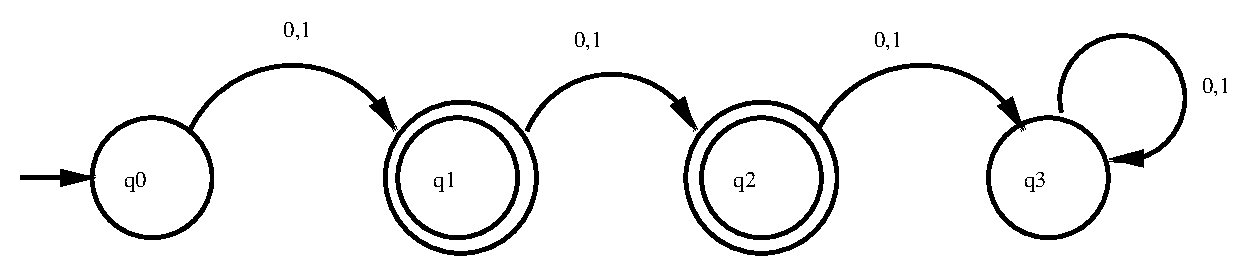
\includegraphics[width=0.5\columnwidth]{figs/dfa2}
}
\end{center}
\end{figure}
For this machine $M_1$, also give its formal description as a 5-tuple. 
You do not need to do this for the machine $M_2$ that follows in part (ii).
\end{enumerate}

\newpage
{\begin{center}\textbf{(continuation of exercise \ref{sec:interpreting})}\end{center}}
\begin{enumerate}[label=(\roman*)]\setcounter{enumi}{1}
\item \textbf{[6 points]}
Please see the DFA of machine $M_2$ below.
\begin{figure}[h]
\begin{center}
{
\psfrag{0}{$0$}\psfrag{1}{$1$}
\psfrag{0,1}{$0,1$}
\psfrag{q0}{$q_0$}\psfrag{q1}{$q_1$}\psfrag{q2}{$q_2$}\psfrag{q3}{$q_3$}
\psfrag{q4}{$q_4$}\psfrag{q5}{$q_5$}\psfrag{q6}{$q_6$}\psfrag{q7}{$q_7$}
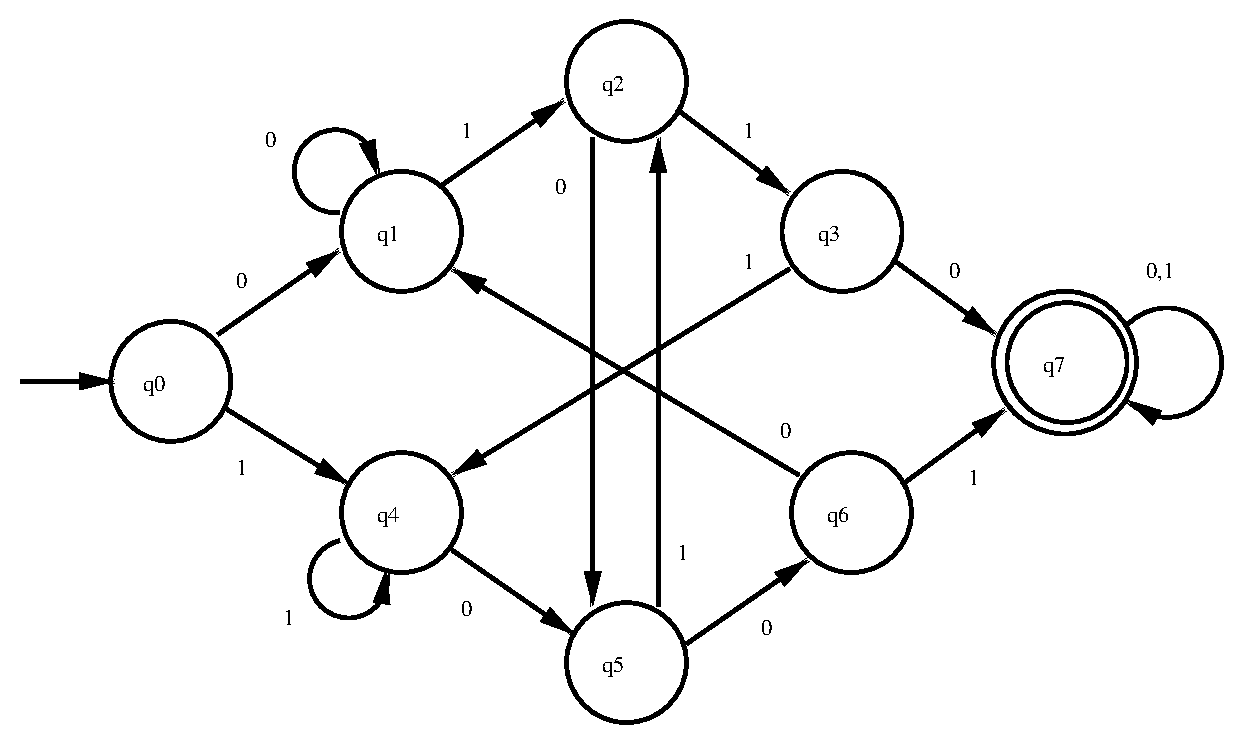
\includegraphics[width=0.5\columnwidth]{figs/dfa3}
}
\end{center}
\end{figure}

\end{enumerate}







\newpage
\section{Closure [4 points]}
Let $A$ and $B$ be regular languages.  Show that $A\setminus B$ is also regular.\\ 
Recall that $A\setminus B = \{x\in A \mid x \not\in B\}$. 
In other words, this operation removes from $A$ all the strings that are also in $B$.








\newpage
\section{Assigned Reading Question [4 points]}
Please read the Quanta article \emph{Computation Is All Around Us, and You Can See It if You Try}, by Lance Fortnow.  The article is available at the link below:
\begin{center}
{\small\href{https://www.quantamagazine.org/computation-is-all-around-us-and-you-can-see-it-if-you-try-20240612/}{https://www.quantamagazine.org/computation-is-all-around-us-and-you-can-see-it-if-you-try-20240612/}}
\end{center}
After reading this article, please answer the question below.

\medskip

\noindent\underline{Question:}
Does Lance Fortnow believe that randomness is unpredictable?  Justify your answer.




\end{document}
